\documentclass{article}
\usepackage{graphicx}
\usepackage{float}
\usepackage[colorlinks=true, urlcolor=blue, linkcolor=black, citecolor=black]{hyperref}
\usepackage[margin=1in]{geometry} % 1 pouce de marge de tous côtés

\title{\textbf{TP Noté}}
\author{TROILLARD Romain \& RELAVE Dorian}
\date{\today}

\begin{document}

\maketitle

\tableofcontents

\newpage

\section{Analyse de l'évolution de la loss pendant l'apprentissage}

Nous avons analysé de manière approfondie l'évolution des fonctions de perte (train et test) lors de l'apprentissage d'un réseau de neurones sur le jeu de données MNIST. Les résultats détaillés de cette analyse sont présentés dans les graphiques suivants, accompagnés d'interprétations.

\subsection{Setup simple}

Pour cette configuration initiale, nous avons appliqué les fonctions telles quelles, en suivant la méthodologie standard qui consiste à effectuer l'entraînement sur un corpus de grande taille et à tester les performances sur un corpus plus restreint.

\begin{figure}[H]
    \centering
    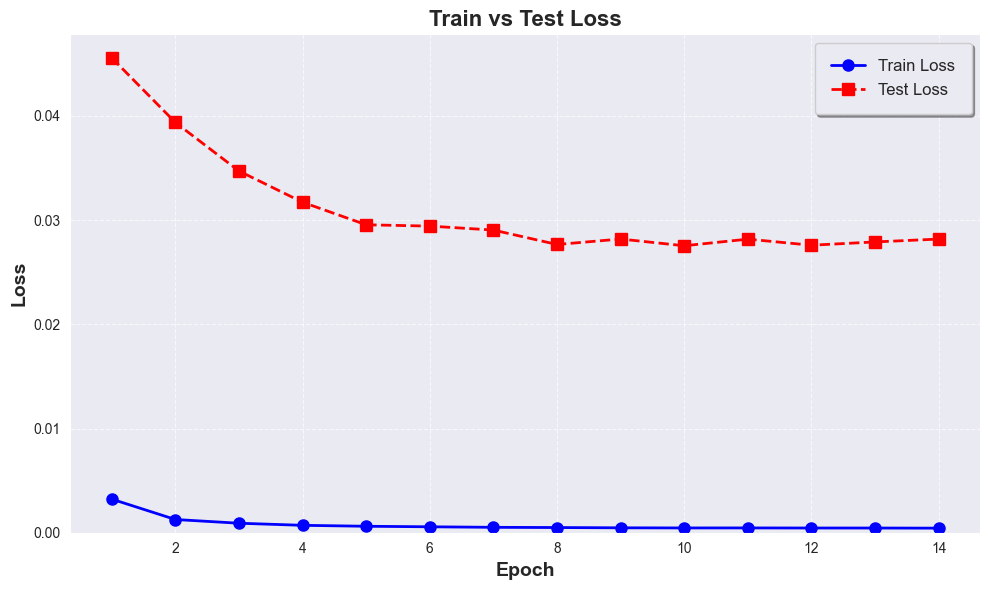
\includegraphics[width=1\textwidth]{train_vs_test.png}
    \caption{Évolution des fonctions de perte (train et test) sur la configuration de base}
    \label{fig:train_vs_test}
\end{figure}

On peut observer sur la figure \ref{fig:train_vs_test} que les deux courbes évoluent de façon décroissante et convergent progressivement vers zéro. On remarque toutefois que cette décroissance ralentit considérablement à partir de la cinquième époque, où les variations deviennent très faibles, indiquant que le modèle atteint un plateau dans son apprentissage.

\newpage
\subsection{Setup inversé}

Pour cette deuxième configuration, nous avons appliqué les mêmes fonctions d'apprentissage, mais en inversant délibérément les données d'entraînement et de test, de sorte que le corpus de test soit plus volumineux que celui d'entraînement. Cette approche non conventionnelle vise à étudier l'impact de la taille des ensembles de données sur l'apprentissage.

\begin{figure}[H]
    \centering
    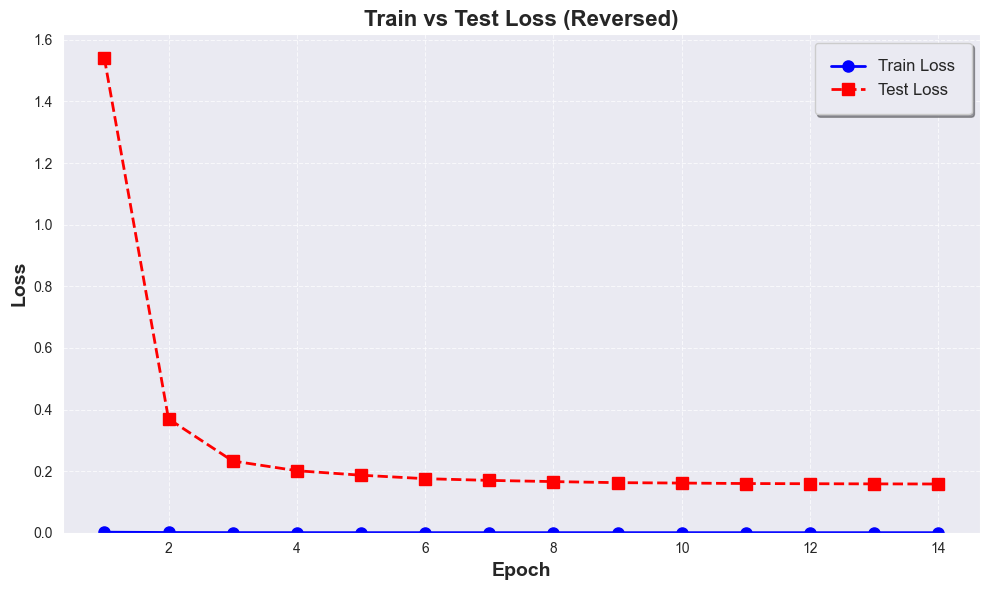
\includegraphics[width=1\textwidth]{train_vs_test_reversed.png}
    \caption{Évolution des fonctions de perte (train et test) sur la configuration inversée}
    \label{fig:train_vs_test_reversed}
\end{figure}

Ce second graphique (\ref{fig:train_vs_test_reversed}) révèle une évolution globalement similaire à celle de la configuration de base. Cependant, on observe une chute particulièrement brutale entre la première et la deuxième époque. Cette discontinuité s'explique par la valeur particulièrement élevée de la fonction de perte lors de la première époque, phénomène directement lié à la taille réduite du jeu de données utilisé pour l'entraînement, qui ne permet pas une initialisation optimale des poids du réseau.

\newpage
\subsection{Setup sans 'Dropout'}
\label{Setup_nd}

Dans le cadre de cette troisième configuration, nous avons délibérément désactivé les fonctions 'Dropout' de la classe \textit{Net} afin d'observer l'impact de cette technique de régularisation.\\
Le \textbf{Dropout} est une technique cruciale en apprentissage profond permettant de réduire le surapprentissage (overfitting) en désactivant temporairement et aléatoirement certains neurones et leurs connexions pendant la phase d'entraînement. Cette méthode force le réseau à développer des caractéristiques plus robustes et moins spécifiques aux données d'entraînement.

\begin{figure}[H]
    \centering
    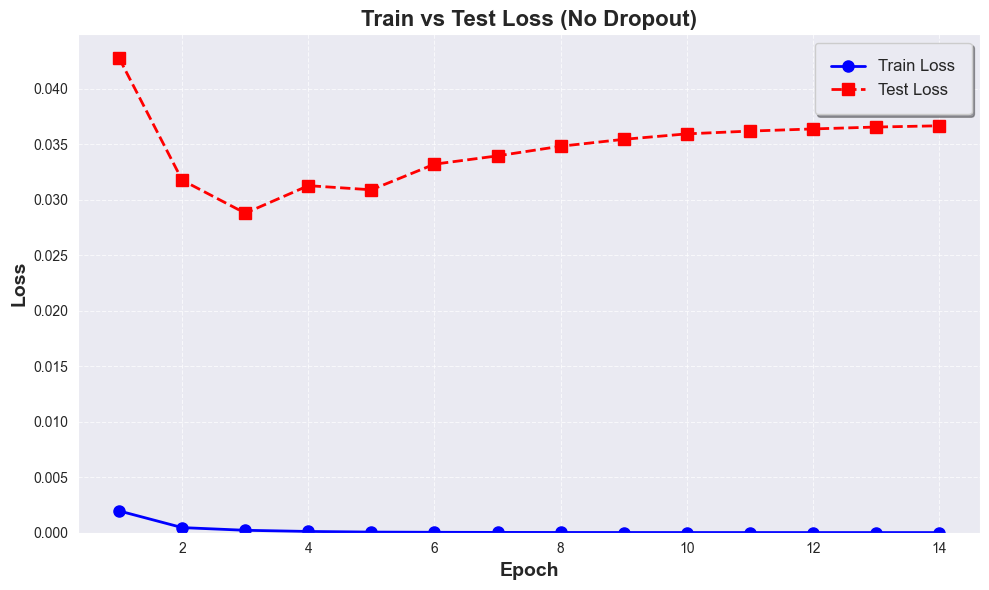
\includegraphics[width=1\textwidth]{train_vs_test_nd.png}
    \caption{Évolution des fonctions de perte (train et test) sans la régularisation par dropout}
    \label{fig:train_vs_test_nd}
\end{figure}

Cette fois-ci, le graphique \ref{fig:train_vs_test_nd} révèle une situation nettement différente et très instructive. Si la courbe d'entraînement (\textit{train}) continue de converger vers zéro comme attendu, on observe en revanche un comportement problématique sur la courbe de test. En effet, à partir de la troisième époque, la fonction de perte sur les données de test augmente continuellement, ce qui constitue un indicateur clair de surapprentissage (overfitting). Le réseau devient progressivement trop spécialisé sur les données d'entraînement et perd en capacité de généralisation sur de nouvelles données, démontrant ainsi l'importance cruciale du dropout comme mécanisme de régularisation.

\newpage
\subsection{Setup inversé et sans 'Dropout'}

Pour cette quatrième et dernière configuration, nous avons combiné les deux modifications précédentes : la désactivation du mécanisme de 'Dropout' et l'inversion des ensembles de données d'entraînement et de test. Cette configuration nous permet d'étudier l'interaction entre ces deux facteurs.

\begin{figure}[H]
    \centering
    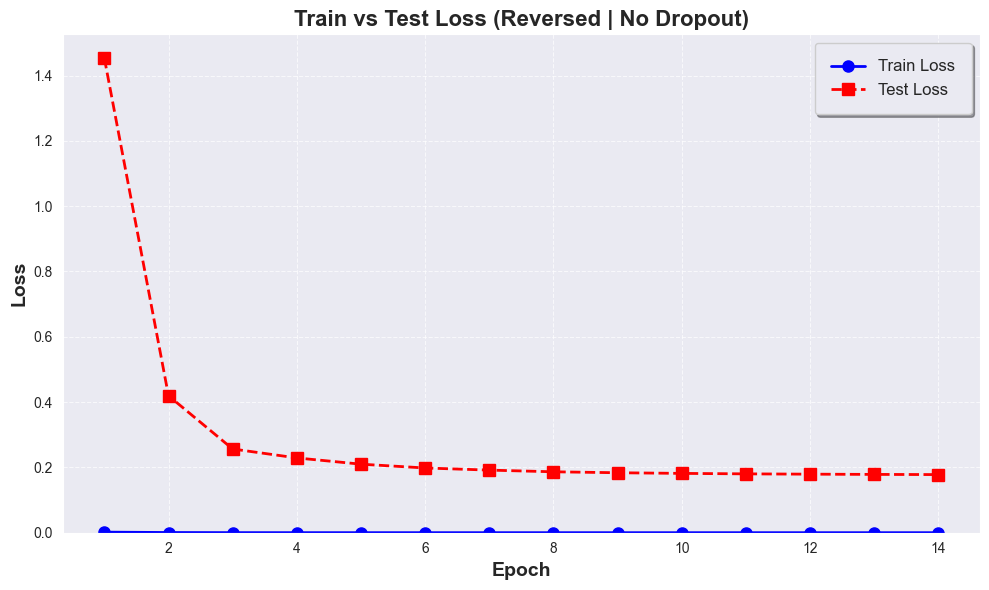
\includegraphics[width=1\textwidth]{train_vs_test_reversed_nd.png}
    \caption{Évolution des fonctions de perte (train et test) avec données inversées et sans régularisation par dropout}
    \label{fig:train_vs_test_reversed_nd}
\end{figure}

Le graphique \ref{fig:train_vs_test_reversed_nd} présente des caractéristiques relativement similaires à celles du graphique \ref{fig:train_vs_test_reversed}, avec notamment une fonction de perte particulièrement élevée lors de la première époque pour les données de test.

\newpage
\subsection{Conclusion}

Afin de tirer des conclusions significatives, nous allons maintenant procéder à une analyse comparative approfondie des différentes configurations expérimentales.

\begin{figure}[H]
    \centering
    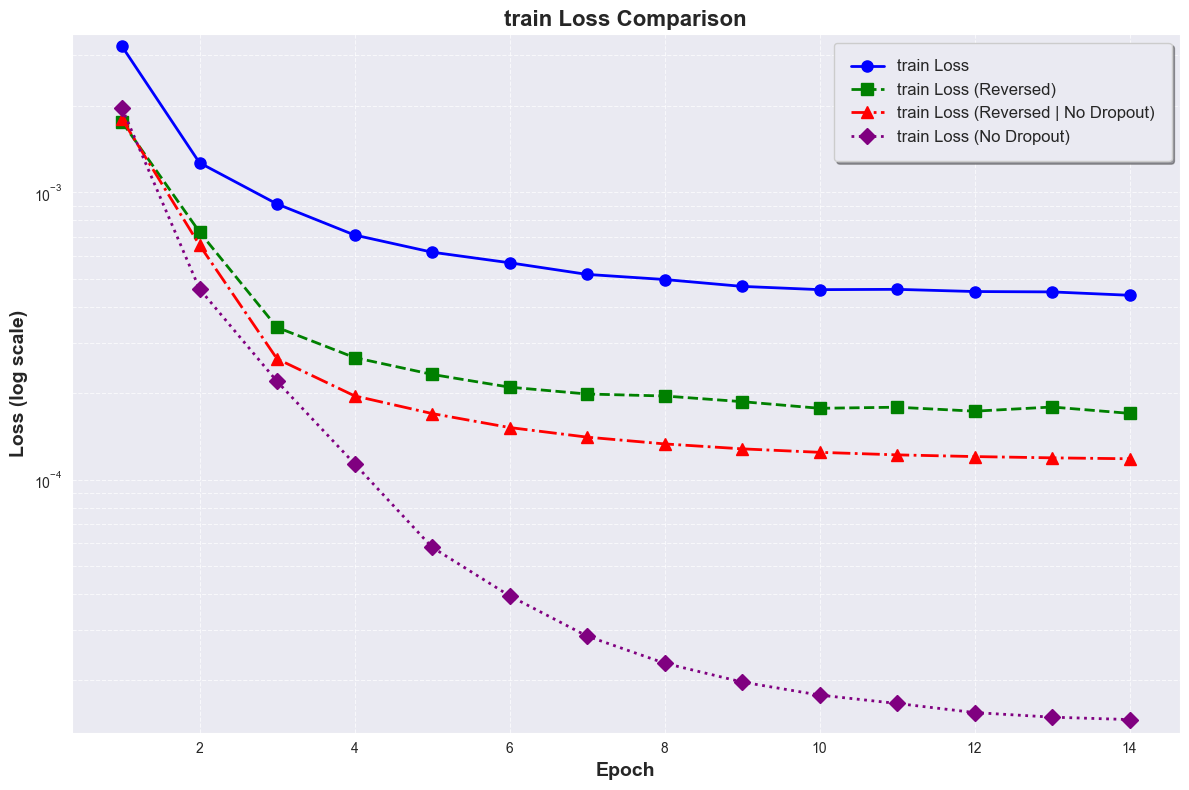
\includegraphics[width=1\textwidth]{train_compare.png}
    \caption{Analyse comparative de l'évolution des fonctions de perte d'entraînement}
    \label{fig:train_compare}
\end{figure}

L'analyse des quatre courbes d'entraînement révèle que toutes les configurations présentent une tendance décroissante de la fonction de perte, ce qui est cohérent avec un processus d'apprentissage fonctionnel. On remarque toutefois que les configurations sans dropout atteignent des valeurs de perte sensiblement plus faibles que les configurations avec dropout. Cette observation est particulièrement intéressante car elle illustre parfaitement le compromis fondamental entre la performance sur les données d'entraînement et la capacité de généralisation du modèle.

\begin{figure}[H]
    \centering
    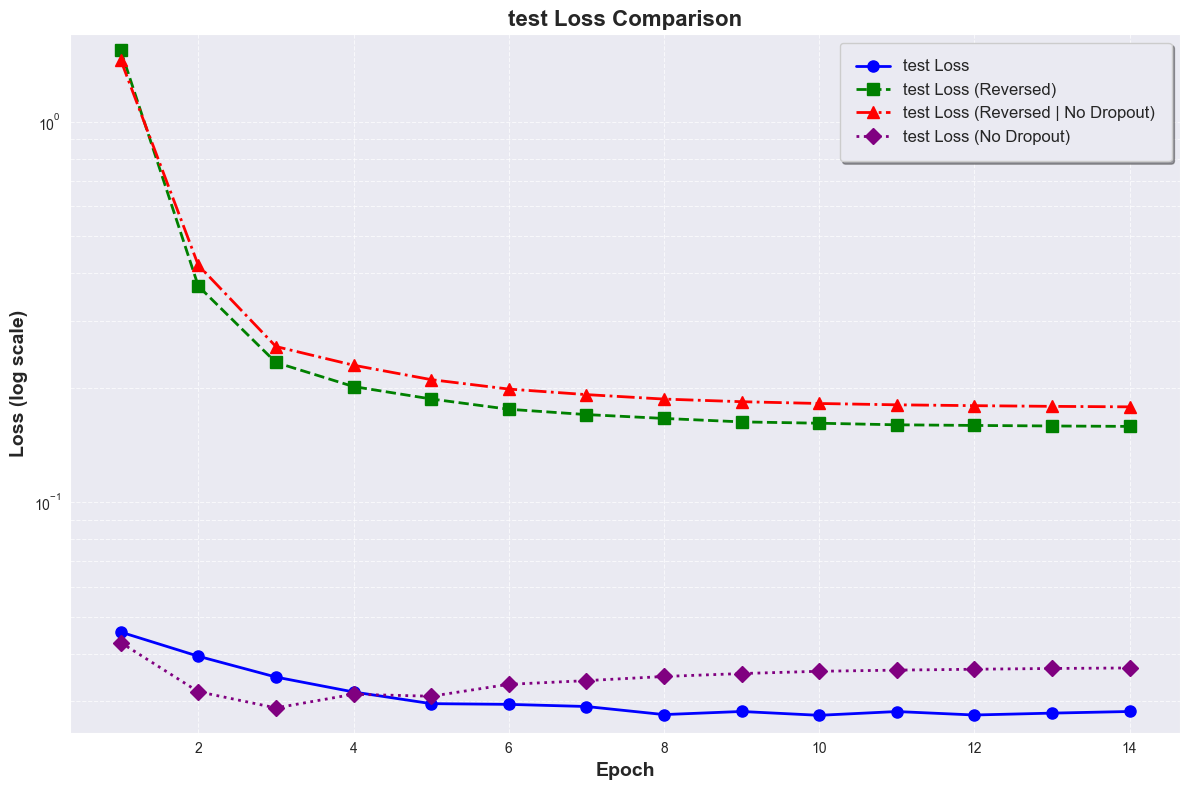
\includegraphics[width=1\textwidth]{test_compare.png}
    \caption{Analyse comparative de l'évolution des fonctions de perte de test}
    \label{fig:test_compare}
\end{figure}

Pour la phase de test, nous observons des résultats très différents. Les configurations avec données inversées montrent des pertes plus élevées que les configurations standards, soulignant l'importance d'avoir un ensemble d'entraînement suffisamment grand. De plus, on remarque que la configuration sans dropout montre une courbe qui remonte, contrairement aux configurations avec dropout qui continuent de descendre vers zéro. Ceci démontre clairement que le dropout joue un rôle essentiel pour éviter le surapprentissage et améliorer la capacité du modèle à généraliser sur de nouvelles données.

En conclusion, cette étude comparative nous permet de dégager plusieurs enseignements fondamentaux :

\begin{itemize}
    \item Lorsque le réseau apprend efficacement, la fonction de perte sur les données d'entraînement diminue progressivement et tend asymptotiquement vers zéro, indiquant une amélioration continue de la capacité prédictive du modèle sur les exemples connus.
    \item La fonction de perte sur les données de test suit généralement une trajectoire similaire dans un apprentissage optimal, mais peut présenter une augmentation significative en cas de surapprentissage (comme clairement démontré dans la configuration \ref{Setup_nd}), signalant une détérioration de la capacité de généralisation du modèle.
    \item L'inversion des ensembles de données d'entraînement et de test s'avère être une stratégie sous-optimale, générant systématiquement des fonctions de perte plus élevées pour la phase de test, ce qui souligne l'importance cruciale d'un ensemble d'entraînement suffisamment riche et représentatif.
    \item Le mécanisme de dropout démontre son efficacité en tant que technique de régularisation, permettant de maintenir une bonne capacité de généralisation au prix d'une légère diminution des performances sur les données d'entraînement, illustrant parfaitement le compromis biais-variance en apprentissage automatique.
\end{itemize}

\end{document}